\chapter{Making predictions using PDFs with theoretical uncertainties}

Earlier in this thesis we have discussed the importance of theoretical uncertainties, and how to include them in PDFs. We have also produced PDFs including MHOUs (see Chapter~\ref{chapter:mhous}) and deuteron and nuclear uncertainties (see Chapter~\ref{chapter:nuclear}), which are freely available. In the future, PDFs with theory uncertainties will become the norm, and will be used widely to make theoretical predictions for observables by convoluting them with parton-level hard cross sections. 

When making predictions for hadronic observables there are two sources of uncertainty: the hard cross section and the PDF. Typically, MHOUs for the former are estimated using scale variation, and these are added in quadrature to the latter. When the PDFs themselves also include MHOUs, we can think of the two scale evolutions considered being $Q_0 \to Q_{dat}$ and $Q_0 \to Q_{pred}$, where $Q_0$ is the PDF parametrisation scale, $Q_{dat}$ is the scale of data in the PDF and $Q_{pred}$ is the scale the prediction is made at. Then each of these sources has both a contribution from renormalisation scale variation and from factorisation scale variation.  The PDFs themselves contain a wealth of data from various processes, so when making a prediction for a process which is included in the PDFs there will invariably be correlations between the renormalisation scale variation in the PDF and that in the hard cross section. Even if the process is a new one, for example Higgs production, correlations due to factorisation scale variation will always be present. Simply combining the two sources of uncertainty in quadrature will miss these correlations and lead to an inflation in overall uncertainties. 

This issue was explored in detail in \cite{Harland-Lang:2018bxd}, noting that PDFs are a tool to express one observable in terms of others. This can be realised exactly in the simple case of fully correlated factorisation scale variation for non-singlet structure functions. Here the PDF can be eliminated entirely, and it is manifest that there is only one independent scale ($Q_{dat} \to Q_{pred}$), rather than two, with the MHOUs cancelling to a large degree. If MHOUs were used in both the PDF and the hard cross section in this case, it would amount to ``double counting". It was also shown that correlations existed for renormalisation scale variation, albeit less strongly.

When using PDFs in predictions we include both sources of scale variation in an uncorrelated way, and so miss the MHOU cancellation and corresponding reduction in uncertainties. As noted in \cite{MHOUbig}, this is a consequence of PDFs being universal. We cannot reconstruct the full data and MHOUs from the PDFs alone as information is lost in the fitting process; one set of PDFs could arise from many different data possibilities. However, if we want PDFs to be useful in a wide range of predictions, universality is required and so we must live with this loss of correlation.

Fortunately, the increase in PDF uncertainties due to MHOUs is small, and the effect is mostly realised in changes to the central value as the fit is rebalanced by changes to the weighting of different data. In indicative cases explored in Chapter 7 of \cite{MHOUbig}, it was seen that the PDF uncertainty is consequently much smaller than the MHOU on the hard cross section. When combining these two in quadrature, the effect of missing correlations will therefore likely be small, and so the overestimate of uncertainty will be small. It was argued that a small overestimate of uncertainty is better than neglecting MHOUs altogether. However, accounting for these correlations is desirable in order to keep uncertainties as low as possible in the current high precision era.

In this chapter we investigate correlations between PDF MHOUs and hard cross section MHOUs when making predictions. Although we focus on MHOUs, the analysis extends naturally to all sources of theory uncertainty. We develop a method for algebraically determining these correlations, and show how to include them when making a prediction. This is a complicated problem so we proceed incrementally:

\begin{itemize}
\item In Sec.~\ref{sec:p1} we show how a theoretical uncertainty can be reformulated in terms of a nuisance parameter, which holds the key to the propagation of uncertainties. We consider as a starting point an exact fit, showing that the experimental data partially decorrelate the theory uncertainties in the fit and those in the prediction.
\item In Sec.~\ref{sec:p2} we move on to a model where the data are fitted using just one parameter. Here the correlations lead to a shift in the theoretical predictions, but the fitting of the data leads to loss of information and consequently further decorrelation.
\item In Sec.~\ref{sec:p3} we extend this analysis to a multi-parameter fit with multiple theory uncertainties, and then to a PDF fit, where the PDFs are continuous functions with a functional uncertainty. We show that this functional uncertainty leads to a further decorrelation in the MHOUs. 
\item In Sec.~\ref{sec:p4} we present numerical results comparing this procedure with the naive approach of adding the uncorrelated contributions in quadrature, in the context of the NLO global fit with MHOUs discussed in Chapter \ref{chapter:mhous}. We make predictions including MHOUs for repetitions of all the experiments already in the fit (so-called ``autopredictions"). We then investigate the scenario of a prediction for a process already in the fit (top production), and for a new process (Higgs production), and show that including these correlations leads to a shift in the central value of the prediction that is well within the total uncertainty, and that the decorrelation of the MHOUs is almost complete. We see that in practice adding the two contributions in quadrature and keeping them uncorrelated (the ``conservative" prescription of Chapter \ref{chapter:mhous}) is remarkably accurate. Having said that, the methodology for including full correlations is now available. Finally, we suggest a novel way of improving theoretical predictions, using ths correlated shift.
\item In Sec.~\ref{sec:p5} we provide a summary.
\end{itemize}

\section{Predictions with correlated theory uncertainties}
\label{sec:p1}

We saw in Chapter \ref{chapter:thuncs} that to include theory uncertainties in a fit all you need to do is add a theory covariance matrix, $S_{ij}$, to the experimental covariance matrix $C_{ij}$. Recall that $i,j = 1, \dots, N_{dat}$ run over data points. The only assumptions underlying this result are that all uncertainties are Gaussian, and that the theory uncertainties are independent of the experimental data. Since Gaussian experimental uncertainties are already assumed in NNPDF's framework, these assumptions are very reasonable. We can express the result as the conditional probability
\be
\label{eqn:ptd}
P(T|D) \propto \exp \bigg( -\frac{1}{2} (T-D)^T(C+S)^{-1}(T-D) \bigg).
\ee
Recall that both $C$ and $S$ are real and symmetric, that $C$ is positive definite and that $S$ is positive semidefinite and will generally possess many zero eigenvalues. In a fit we determine $T$ from $D$ by maximising $P(T|D)$, which amounts to minimising
\be
\label{eqn:chi2}
\chi^2 =  (T-D)^T(C+S)^{-1}(T-D)
\ee
with respect to the free parameters which characterise the theory prediction.

In this section we start off by considering one single source of fully correlated theory uncertainty, so that
\be 
S = \beta \beta^T,
\ee
where $\beta$ are real and non-zero. 

\subsection{Nuisance parameters}
We can model the theory uncertainty as a fully correlated shift in the theory prediction:
\be 
T \to T + \lambda \beta,
\ee 
where $\lambda$ is a nuisance parameter characterising the scale of the shift. We will now show that this will lead us to Eqn.~\ref{eqn:ptd}. Firstly, assuming Gaussian experimental uncertainties, we can write
\be 
\label{eqn:nuisptd}
P(T|D\lambda) \propto \exp \bigg( -\frac{1}{2} (T + \lambda \beta -D)^T C^{-1}  (T + \lambda \beta -D) \bigg).
\ee
Using Bayes' Theorem, 
\be 
\label{eqn:bayes}
P(T|D\lambda) P(\lambda |D) = P(\lambda | TD)P(T|D).
\ee
We want to find $P(T|D)$, so we need an expression for the prior for $\lambda$, $P(\lambda |D) = P(\lambda)$, where we assume that the theory uncertainty is independent of the experimental data. We choose a unit-width Gaussian centred on zero, 
\be 
\label{eqn:lambdaprior}
P(\lambda) \propto \exp \bigg(-\frac{1}{2} \lambda^2 \bigg).
\ee
Marginalising over $\lambda$, Eqn.~\ref{eqn:nuisptd} becomes
\be 
\label{eqn:ptd2}
P(T|D) \propto \int d\lambda \exp \bigg( -\frac{1}{2} \bigg[ (T + \lambda \beta -D)^T C^{-1} (T + \lambda \beta -D) + \lambda^2 \bigg] \bigg).
\ee
We can evaluate the term in $[ \cdot ]$ by remembering $S= \beta \beta^T$, introducing the variable
\be 
\label{eqn:z}
Z \equiv (1 + \beta^T C^{-1} \beta)^{-1},
\ee
and completing the square:
\be 
\begin{split}
[ \cdot ] &= (T-D)^T C^{-1}(T-D) + (T-D)^T C^{-1} \lambda \beta + \lambda \beta^T C^{-1} (T-D) \\ &+ \lambda \beta^T C^{-1} \lambda \beta + \lambda^2 \\
& = (T-D)^T C^{-1}(T-D) + (T-D)^T C^{-1} \lambda \beta + \lambda \beta^T C^{-1} (T-D) + \lambda^2 Z^{-1} \\
&=  Z^{-1}(\lambda + Z \beta^T C^{-1} (T-D))^2 \\ &- Z(\beta^T C^{-1} (T-D))^2 + (T-D)^T C^{-1}(T-D) \\
&= Z^{-1}(\lambda + Z \beta^T C^{-1} (T-D))^2 \\ &+ (T-D)^T (C^{-1} - Z C^{-1} S C^{-1})(T-D).
\end{split}
\ee
Finally, we can use the Sherman-Morrison formula and Eqn.~\ref{eqn:chi2} to write this as
\be 
\begin{split}
[ \cdot ] &= Z^{-1}(\lambda + Z \beta^T C^{-1} (T-D))^2 + (T-D)^T (C + S)^{-1}(T-D) \\
&= Z^{-1}(\lambda + Z \beta^T C^{-1} (T-D))^2 + \chi^2 \\
&\equiv Z^{-1}(\lambda - \bar{\lambda}) + \chi^2,
\end{split}
\ee
where we have defined $\bar{\lambda} = Z \beta^T C^{-1} (D-T)$. Plugging this back into Eqn.~\ref{eqn:ptd2}, we get
\be  
\begin{split}
P(T|D) &\propto \int d\lambda \ e^{-\frac{1}{2} \chi^2} \exp \bigg( -\frac{1}{2} Z^{-1} (\lambda - \bar{\lambda})^2 \bigg) \\
&\propto e^{-\frac{1}{2} \chi^2},
\end{split}
\ee
which is Eqn.~\ref{eqn:ptd}. The advantage of this approach is that we can also get the posterior distribution for $\lambda$ (after fitting using $D$ and $T$), by using Bayes' Theorem (Eqn.~\ref{eqn:bayes}):
\be 
\begin{split}
\label{eqn:lambdaposterior}
P(\lambda |TD) &= \frac{P(T|D\lambda) P(\lambda)}{P(T|D)} \\
&= \exp \bigg( -\frac{1}{2} \bigg[ (T+ \lambda \beta -D)^T C^{-1}(T+ \lambda \beta -D) + \lambda^2 - \chi^2 \bigg] \bigg) \\
& = \exp \bigg( -\frac{1}{2} Z^{-1}(\lambda - \bar{\lambda})\bigg),
\end{split}
\ee
where we recognised the similarity between the exponent here and in Eqn.~\ref{eqn:ptd2}. So the effect of the fit is to shift the centre of the distribution from 0 $\to \bar{\lambda}$, and the width from 1 $\to Z$. Note that from the definition of $Z$ (Eqn.~\ref{eqn:z}), 
\be 
0 \le Z \le 1,
\ee
so the theory uncertainty is always reduced when information on $D$ is added. Fig.~\ref{fig:lambdadistribs} gives a sketch of this effect.  
%%%%%%%%%%%%%%%%%%%%%%%%%%%%%%%%%%%%%%%%%%%%%%%%%%%%%%%%%%%%%%%%%%%%%
\begin{figure}[H]
  \begin{center}
      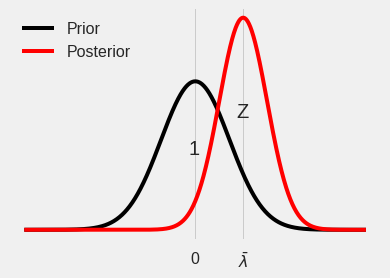
\includegraphics[width=0.5\textwidth]{correlations/plots/lambdapriorpost.png}
    \caption{Sketch of the prior (Eqn.~\ref{eqn:lambdaprior}) and posterior (Eqn.~\ref{eqn:lambdaposterior}) distributions for $\lambda$. Adding information shifts the distribution and reduces the width. \label{fig:lambdadistribs}}
    
  \end{center}
\end{figure}
%%%%%%%%%%%%%%%%%%%%%%%%%%%%%%%%%%%%%%%%%%%%%%%%%%%%%%%%%%%%%%%%%%%%%%

\section{Predictions from one-parameter fits}
\label{sec:p2}

\section{Correlated MHOUs in PDF fits}
\label{sec:p3}

\section{Numerical results}
\label{sec:p4}

\section{Summary}
\label{sec:p5}
